\section{Analysephase}
\label{sec:Analysephase}
%TODO:Quelle Recherche Problemdefinition / Requiremants Engeneering
Die Analysephase eines Softwareentwicklungsprojekts spielt eine entscheidende Rolle für den Erfolg eines Projekts, da hier die Anforderungen an das zu entwickelnde System erhoben werden. Zur Ermittlung der Anforderungen soll eine Datenanalyse und eine Anforderungsanalyse durchgeführt werden, die Einblicke in die bisherigen Prozesse der Anwesenheitsplanung geben sollen. Für die Informationsbeschaffung wird auf die Analysemethode der Datenanalyse gesetzt. Um die so gewonnenen Daten zu Validieren und auch subjektive Verbesserungsvorschläge zu berücksichtigen werden Intervierws mit den Mitarbeitern durchgeführt. Die dabei erhobenen Daten werden dann Aufbereitet und zu modellierung von Spezifikationen genutzt. Modelle bei der Softwareentwicklung werden genutzt um Anforderungen in für den Auftraggeber und den Entwickler interpretierbarer Form darzustellen. (vgl. \cite[S. 43]{dumke-2003})

Die folgenden Abschnitte beschreiben die Vorgehensweise und Ergebnisse der durchgeführten Analysen. Die dabei gewonnenen Erkenntnisse bilden die grundlage für die weiteren Entscheidungen für die Umsetzung des Projektes.


\subsection{Analyse des Ist-Zustandes}
\label{sec:Ist-Zustand}
% Bestehende Anwesenheitsplanungsmethoden (Datenstruktur/Tabellenaufbau)
% Schwachstellen und Herausforderungen im aktuellen Prozess
Um eine verbesserte Variante eines Anwesenheitsplaners zu erstellen ist es notwendig die bestehenden Systeme und Abläufe zu verstehen. Dafür wurden Interviews mit Mitarbeitern aus verschiedenen Referaten geführt und analog dazu die verschiedenen Excel-Dateien analysiert. Dabei lag der Fokus auf der Analyse des Prozesses der Anwesenheitsplanung, um diesen durch die neue Variante des Anwesenheitsplaners bestmöglich zu unterstützen.

Die Interviews ergaben, dass das Excel-Dokument meist in einem Netzlaufwerk aufbewahrt wird um für die Rederatsmitglieder zugänglich zu sein. Das Dokument wird nicht anders behandelt als andere Referatsdaten was bedeutet, dass es keine spezielle Rechteverwaltung gibt. Das kann zu Fehlern und Inkonsistenzen durch versehentliches ändern anderer Datensätze führen, da jeder im referat schreibrechte auf das ganze Dokument hat.

Als größte Problem wurde die Tatsache, dass nur ein Nutzer gleichzeitig auf das Excel-Dokument zugreifen kann festgestellt. Dies führt dazu, dass für eine unbestimmte Zeit keine Möglichkeit besteht den eigenen Status zu ändern. Meistens tritt der Umstand auf, wenn ein Mitarbeiter die Datei im Hintergrund geöffnet hat diese aber nicht nutzt.

Für die Datenanalyse wurden von den beteiligten Referaten eine Kopie ihrer Excel Datei zur Verfügung gestellt. Hauptsächlich sollte der grafische Aufbau der Tabelle und die enthaltenen Informationen der Tabellen untersucht werden. Die Analyse ergab, dass alle Anwesenheitsplaner Tabellen ähnlich aufgebaut sind. Unterschiede ergaben sich meist nur in der Bezeichnung der Anwesenheitszustände und die Granularität der Zeitabschnitte. Um eine Referenz für die weitere Entwicklung zu haben wurde aus den Referats-Tabellen eine Modelltabelle für die Anwesenheitsplanung erstellt, siehe \ref{abb:Ausgangstabelle}.

Basierend auf diesen Erkenntnissen wird deutlich, dass der Anwesenheitsplaner an vielen Stellen verbessert werden muss. Die neue Lösung sollte die Möglichkeit bieten, dass mehrere Nutzer gleichzeitig auf die Anwesenheitsdaten zugreifen und diese aktualisieren können. Die Automatisierung von Prozessen und die Integration einer Datenbank könnten die Genauigkeit, Effizienz und Benutzerfreundlichkeit des Anwesenheitsplaners erheblich verbessern.

\subsection{Anforderungen an den Anwesenheitsplaner}
\label{sec:Soll-Zustand}
%TODO:Berechtigungensonzept
Basierend auf den in der Ist-Analyse gesammelten Erkenntnissen wird deutlich, dass der Anwesenheitsplaner an vielen Stellen verbessert werden muss. Um die zu Anforderungen an das neue System darzustellen wurde eine Use-Case-Analyse durchgeführt. Dabei wird das gewünschte Verhalten der Software dem Nutzer gegenüber als Anwendungsfall spezifiziert. Aus der Summer aller Nutzungsfälle lässt sich dann die gewünschte Funktionalität der Software ableiten ohne dabei auf konkrete Realisierungsschritte eingehen zu müssen.(vgl. \cite[S. 164]{neumann-2002})

\begin{figure}[htb]
    \centering
    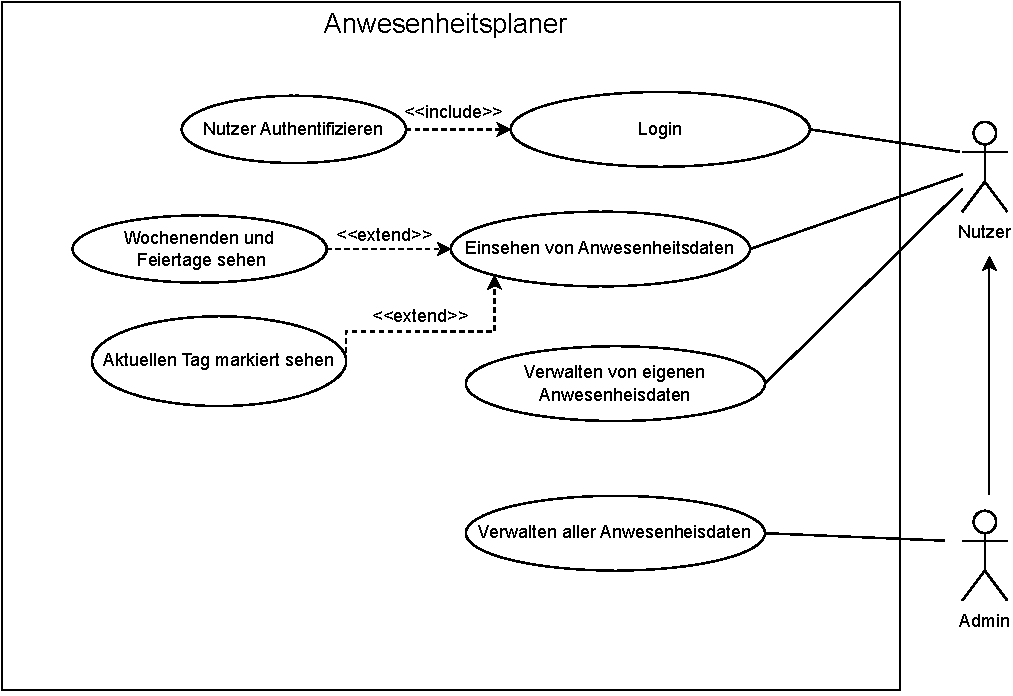
\includegraphics[width=0.7\textwidth,angle=0]{abb/use-case-diagramm.pdf}
    \caption[Beschreibung]{Use-Case-Diagramm}
    \label{fig:Use-Case-Diagramm}
\end{figure}

Aus dem Use-Case-Diagramm in Abbildung~\ref{fig:Use-Case-Diagramm} geht hervor, das ein Nutzer sich am System anmelden können soll um Anwesenheitsdaten seines Referates zu sehen und eigene Daten zu verwalten. Das Verwalten soll das erstellen, bearbeiten und löschen von Einträgen beinhalten. Desweiteren wird auch einen zweiten Nutzertyp benötigt, der als Admin fungiert und Einträge von anderen Mitarbeitern des Referates ändern kann.

Aus den Intervierws konnten noch weitere Spezifikationen ermittelt werden. Am wichtigsten ist die Möglichkeit zu Mehrbenutzerzugriff. Die neue Software sollte es ermöglichen, dass mehrere Benutzer gleichzeitig auf den Anwesenheitsplaner zugreifen und ihre Daten aktualisieren können. Dadurch werden Engpässe bei der Aktualisierung der Anwesenheitsdaten vermieden und die Benutzerfreundlichkeit verbessert. Um die Benutzerfreundlichkeit noch weiter zu Verbessern soll eine ähnliche Benutzeroberfläche wie in der Excel Liste entstehen, jedoch das Eintragen der Datensätze, durch \zB Mehlfachauswahl vereinfacht.

Zudem sollen Datenschutz und Datensicherheit im neuen System gewährleisten werden. Dafür werden Sicherheitsmaßnahmen benötigt die vor unbefugtem Zugriff oder Verlust der Daten schützen. Dafür werden Mechanismen zur Datensicherung und Benutzer-Authentifizierung benötigt, um zu gewährleistet, dass Benutzer nur auf die Daten zugreifen und Änderungen vornehmen können, für die sie autorisiert sind.

Um den geforderten Systemaufbau modellhaft zu Skizzieren wurde ein Paketdiagramm erstellt. Dieses soll für die Entwurfsphase als Referenz genutzt werden.

\begin{figure}[htb]
    \centering
    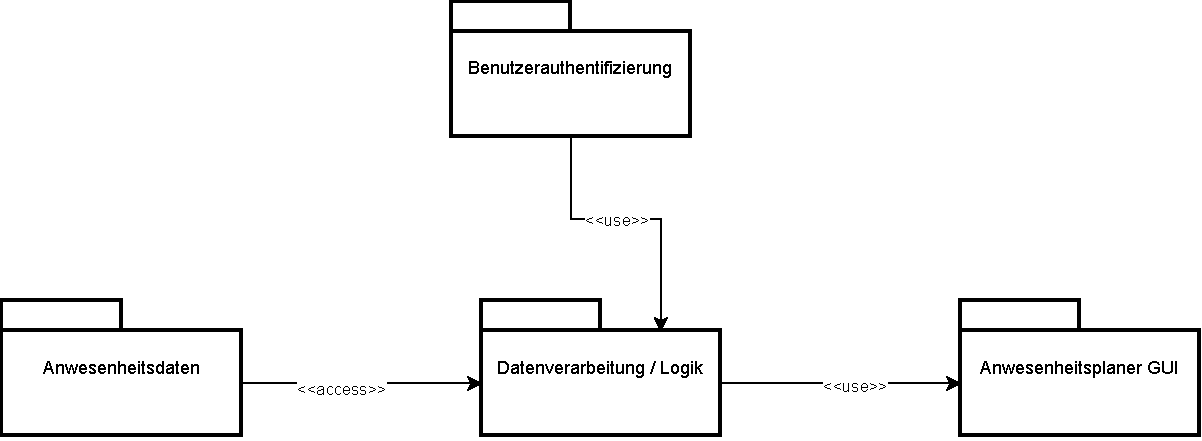
\includegraphics[width=0.7\textwidth,angle=0]{abb/Paketdiagramm.pdf}
    \caption[Beschreibung]{Paketdiagramm}
    \label{fig:Paketdiagramm}
\end{figure}

\subsection{Datenschutz und Datensicherheitsanalyse}
\label{sec:Datenschutz}
%TODO:Personenbezogene Daten?
%TODO:Anforderungen Datenschutzkonzept
%TODO:Datensicherheit / Risikoanalyse